\chapter{常见误区}
\label{chap:e27}

\begin{chapteropening}
一本书讲到这里，工具箱已经装满了：泊松统计、相干态与热态、\(g^{(1)}\) 与 \(g^{(2)}\)、Siegert 关系、强度干涉、SPADE、Fisher 信息、事件表与相关器。可越是工具趁手，越容易在最后一公里踩坑——把"数到了光子"当成"做了量子天文学"，把 \(g^{(2)}\simeq1\) 当成"这是激光"，把一次偶然的高计数当成"新物理"。这些坑有一个共同点：它们都在\emph{正确结论的隔壁}，差一步就掉进去。本章不引入任何新公式的物理内容，而是把前面各章已经严格建立的结论，一条一条摆到"最容易误读它"的场景旁边，讲清楚每个误区\textbf{错在哪、正确的物理图像是什么}。读完这一章，你手里的工具不会变多，但你用错它们的概率会明显变小。
\end{chapteropening}


\section{"数到了光子"为什么不等于"做了量子天文学"}
\label{sec:e27-photon-not-quantum}

先说一个最普遍、也最隐蔽的误会：只要探测器能一个一个地"数出"光子，就以为自己已经站在了量子天文学的门里。

单光子探测器（single-photon detector）确实是入口，但它只是入口。第 \ref{chap:e13} 章讲过，一台会数光子的仪器交给我们的原始产物，是一张\textbf{事件表}（event list）：每一行记一个被探测到的光子，带着它的到达时间 \(t\)（单位 s 或 ns）、探测器/望远镜编号 \(d\)、频率通道 \(\nu\)（单位 Hz 或通道号）、偏振标签 \(p\)。这张表里\emph{可能}藏着量子信息，但藏没藏、取没取出来，取决于你后面怎么处理它。

设想两种处理方式。第一种：把事件表按时间分箱，数每个箱里有多少行，得到一条计数率曲线
\[
  R=\frac{N_\gamma}{T},
\]
其中 \(N_\gamma\) 是总光子数，\(T\) 是观测时长（s），\(R\) 的单位是 \({\rm s}^{-1}\)。这就是一条普普通通的光变曲线，和一百年前用照相底片测的星等曲线没有本质区别——你只是用更贵的仪器，重新数了一遍"平均有多亮"。第二种：不去数总量，而去问事件\emph{彼此之间}的关系——两个探测器、两个时间门里的光子是不是比巧合更爱一起响。这才是第 \ref{chap:e08} 章的 \(g^{(2)}\)、第 \ref{chap:e10} 章的强度干涉、第 \ref{chap:e12} 章的模式测量在做的事。判据非常干脆：\textbf{看那些标签有没有真正进入模型}。如果 \(t,d,\nu,p\) 在分析时全被求和抹掉，只剩一个平均率，那么无论探测器多先进，你做的都还是经典测光。

这里要顺手拆掉一个孪生的误会：把"光子数很少"直接等同于"量子"。X 射线和伽马射线天文学几十年来一直在低光子数下工作，用泊松计数和 Cash 似然做谱拟合 \citep{1979ApJ...228..939C,1986ApJ...303..336G}，但这些分析的目标绝大多数仍是平均强度或能谱——是经典量，只不过噪声模型是泊松的而已。反过来，射电和毫米波常常处在\emph{高}占有数、近经典的波动极限，却照样能严肃地讨论相干函数、相位、偏振和量子噪声。可见"少光子"与"量子"是两把不同的尺子：区分的关键不在光子多少，而在\textbf{模型是否需要多光子的联合概率或光场模式来表达}。

还有第三个连带的坑：以为"有了事件表就会自动冒出新物理"。不会。第 \ref{chap:e03} 章的泊松模型摆在那里：一段观测里第 \(k\) 个箱的计数期望是
\[
  \mu_k=R_k\,E_k\,\Delta t_k,
\]
其中 \(R_k\) 是该箱的瞬时率（\({\rm s}^{-1}\)），\(\Delta t_k\) 是箱宽（s），\(E_k\) 是无量纲的有效曝光因子（把云、死时间、选择函数一并吸收进来），\(\mu_k\) 本身无量纲。一个常见的错误操作是：把所有 \(N_k\) 和\emph{同一个}常数 \(\mu\) 去比，发现方差偏大，就宣布"非泊松、有新物理"。可只要源本来就在变（\(R_k\) 随时间变），或者天气、死时间让 \(E_k\) 在变，\(\mu_k\) 就本该逐箱不同——你比的那个"常数 \(\mu\)"从一开始就是错的基准。真正要做的是让模型把这些普通的变化吃进去，再看残差。Bayesian Blocks、周期搜索、似然比检验都能处理这类问题，但每一种都有自己的适用条件和试验次数 \citep{2013ApJ...764..167S,1982ApJ...263..835S,1992ApJ...398..146G,2002ApJ...571..545P}——这一点会在本章最后一节回来算账。

一句话收束这一节：\textbf{能数光子只是拿到了原料，量子天文学的新信息藏在事件之间的联合分布里；标签不进模型，光子数得再准也白搭。}


\section{\texorpdfstring{为什么 \(g^{(2)}\simeq1\) 说明不了问题}{为什么 g2 约等于 1 说明不了问题}}
\label{sec:e27-g2}

第二个坑几乎是量子光学入门者的"必踩项"：看到 \(g^{(2)}(0)\simeq1\)，要么脱口而出"这是相干激光"，要么反过来断言"没有任何量子性"。两种说法都站不住。

先把第 \ref{chap:e08} 章的严格结论摆出来。相干态（coherent state，理想单模激光的模型）确实给出泊松光子数分布和 \(g^{(2)}(0)=1\)。但这句话不能反过来读：\(\mathbf{g^{(2)}(0)=1}\) \textbf{并不是相干态的唯一指纹}。热光（thermal light，恒星那样的混沌光源）单模时 \(g^{(2)}(0)=2\)，可一旦有很多模式叠加、或者探测器把远短于自己响应时间的相干涨落平均掉，那个高出 1 的"聚束峰"（bunching peak）就会被迅速稀释，测出来的 \(g^{(2)}(0)\) 会无限接近 1。也就是说，\(g^{(2)}\simeq1\) 既可能是真正的相干光，也可能是被稀释得面目全非的热光——单凭这个数，你分不出是哪一种。

把稀释写成公式，物理图像就清楚了。第 \ref{chap:e08} 章给过对比度稀释的基本形式，这里用它的实用版本：

\begin{equation}
  g^{(2)}_{\rm meas}(0)-1
  \;\simeq\;
  \frac{g^{(2)}_{\rm src}(0)-1}{M_{\rm eff}},
  \qquad
  M_{\rm eff}\simeq M_\perp\,M_\nu\,M_{\rm pol}\,\frac{\Delta t_{\rm eff}}{\tau_c}.
  \label{eq:e27-dilution}
\end{equation}
\begin{formulaexplain}
\(g^{(2)}_{\rm src}\) 是光源本身的二阶相干（热光单模为 2），\(g^{(2)}_{\rm meas}\) 是探测器实际测到的；\(M_{\rm eff}\) 是相关箱内被平均掉的有效模式数，\(M_\perp,M_\nu,M_{\rm pol}\) 分别是空间、频率、偏振模式数，\(\Delta t_{\rm eff}/\tau_c\) 是被抹平的时间模式数。模式越多，聚束峰被压得越低。
\end{formulaexplain}

逐个符号落实并代真实数字。式子右边的分子 \(g^{(2)}_{\rm src}(0)-1\) 对单模热光等于 1（无量纲），是"没被稀释时的满格对比度"。分母 \(M_{\rm eff}\) 是无量纲的有效模式数，它把四种平均一并算进来：空间上望远镜若同时收了源的多个相干斑，\(M_\perp>1\)；频率上滤光片放进了多个相干带宽，\(M_\nu>1\)；偏振若不做选择，\(M_{\rm pol}\approx2\)；而时间上，探测器的响应或相关箱宽 \(\Delta t_{\rm eff}\)（s）远大于相干时间 \(\tau_c\)（s），就把 \(\Delta t_{\rm eff}/\tau_c\) 段互不相干的波列平均成一段。

现在代数字。第 \ref{chap:e08} 章用 \(\tau_c\simeq1/\Delta\nu=\lambda^2/(c\,\Delta\lambda)\) 算过：一片 \(1\,{\rm nm}\) 的窄带滤光片在 \(500\,{\rm nm}\) 附近给 \(\tau_c\sim0.8\,{\rm ps}\)（\(\Delta\nu\sim1.2\times10^{12}\,{\rm Hz}\)）；若滤光片放宽到 \(10\,{\rm nm}\)，带宽增大十倍，\(\tau_c\) 也缩到十分之一，约 \(8\times10^{-14}\,{\rm s}\)、即 \(10^{-13}\,{\rm s}\) 量级。而快电子学的相关箱通常在 \(\Delta t_{\rm eff}\sim10^{-9}\)--\(10^{-8}\,{\rm s}\)。于是仅时间一项就贡献
\[
  \frac{\Delta t_{\rm eff}}{\tau_c}\sim\frac{10^{-9}}{10^{-13}}
  =10^{4}
  \quad\text{到}\quad
  \frac{10^{-8}}{10^{-13}}=10^{5}.
\]
即便空间、频率、偏振都做到"单模"（\(M_\perp=M_\nu=M_{\rm pol}=1\)），测到的对比度也只有
\[
  g^{(2)}_{\rm meas}(0)-1\sim\frac{1}{10^{4}\text{--}10^{5}}
  \sim10^{-4}\text{--}10^{-5},
\]
再叠上多模因子，落到 \(10^{-5}\)--\(10^{-6}\) 是常态。所以恒星热光的 \(g^{(2)}(0)\) 测出来\emph{本来就该}贴着 1，高出的那一点点是要在小数点后第五、第六位上找的信号。Guerin 团队的星光聚束实验、AQuEye/IquEye 方案、VERITAS 与 MAGIC 的强度干涉，都把这个稀释当成\emph{核心量}来对待，而不是当成"没量子性"的证据 \citep{2017MNRAS.472.4126G,2016SPIE.9907E..0NZ,2020NatAs...4.1164A,2021MNRAS.506.1585Z,2024MNRAS.529.4387A,2024ApJ...966...28A}。图 \ref{fig:e27-g2-scaling} 把这条稀释链画了出来。

\begin{figure}[tbp]
\centering
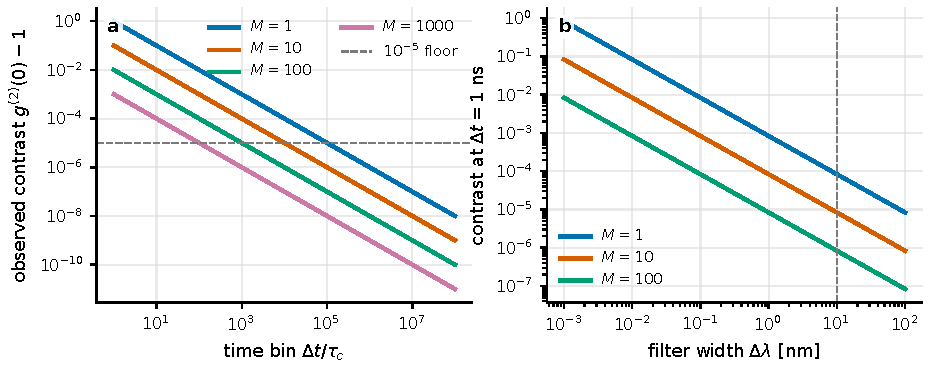
\includegraphics[width=0.96\linewidth]{figures/generated/chapter_21/ch21_g2_scaling_mistake.pdf}
\caption{时间箱、光谱带宽和模式数如何把 \(g^{(2)}\) 的对比度稀释。左图显示 \(\Delta t/\tau_c\) 和 \(M_{\rm eff}\) 怎样把单模热光的聚束峰一路压低；虚线标出 \(10^{-5}\) 量级的系统误差地板。右图把滤光片带宽换算成相干时间：在 \(1\,{\rm ns}\) 采样下，宽带可见光的热光峰很容易低到可校准范围之下。这正是"\(g^{(2)}\simeq1\)"的真实来历——不是没有量子性，而是量子性被平均稀释了。}
\label{fig:e27-g2-scaling}
\end{figure}

那么什么才是\textbf{真正过硬的非经典判据}？答案是反聚束（antibunching），即
\[
  g^{(2)}(0)<1.
\]
第 \ref{chap:e08} 章证明过：任何经典的随机强度都满足 \(g^{(2)}(0)\ge1\)（这是柯西–施瓦茨不等式的直接后果），所以 \(g^{(2)}(0)<1\) 是经典光\emph{无论如何也做不到}的事——它意味着光子彼此"回避"，是单量子发射体的标志。Kimble、Dagenais 和 Mandel 的共振荧光实验，就是靠测到 \(g^{(2)}(0)<1\) 才第一次坐实了反聚束 \citep{1977PhRvL..39..691K}。但要在天体光源里看到反聚束近乎不可能：天体的光通常是海量独立发射体、无数传播路径、有限探测器响应混在一起的结果，任何单个量子发射体的亚泊松特征，都会被式 \eqref{eq:e27-dilution} 里那个巨大的 \(M_{\rm eff}\) 稀释到看不见。

于是这一节的教训是双向的：一篇天文报告若写"\(g^{(2)}\simeq1\)，所以这是激光"，或写"\(g^{(2)}\simeq1\)，所以没有量子信息"，两句都没有依据。\(\mathbf{g^{(2)}\simeq1}\) \textbf{是被稀释后的默认结果，它既不证明相干、也不否证量子；只有 }\(\mathbf{g^{(2)}(0)<1}\)\textbf{ 才是不可辩驳的非经典证据。}


\section{强度干涉为什么依然离不开校准}
\label{sec:e27-calibration}

第三个坑源于对强度干涉一个真实优点的过度乐观。第 \ref{chap:e10} 章讲过，强度干涉（intensity interferometry）测的是两路强度涨落的相关，对大气整体相位（piston，即两路光程共同的平移相位）不敏感——这是它相对振幅干涉最大的工程优势，也是 Hanbury Brown 和 Twiss 当年能在 Narrabri 用简陋镜面测出恒星角直径的原因 \citep{1956Natur.178.1046H,1957RSPSA.242..300B,1974iiia.book.....H}。可"不怕相位"很容易被误读成"不怕误差"。事实恰恰相反：因为要找的信号已经被稀释到 \(10^{-5}\) 量级（上一节），任何一个同样量级的\emph{幅度}误差都能把结论掀翻。

把实际测到的相关超额写成一个数据模型，就能看清有哪些项在捣乱：

\begin{equation}
  \hat c_b(\tau)=
  \beta_b\,|V_b|^2\,h_b(\tau)
  +c_{{\rm inst},b}(\tau)
  +c_{{\rm sel},b}(\tau)
  +\epsilon_b(\tau).
  \label{eq:e27-calibration-model}
\end{equation}
\begin{formulaexplain}
\(\hat c_b=\hat g_b^{(2)}-1\) 是基线 \(b\) 上测到的归一化相关超额。第一项是真正的天体信号，后面依次是仪器项、选择项、随机误差。强度干涉不怕大气\emph{相位}，却照样怕这些\emph{幅度}项。
\end{formulaexplain}

逐项拆开，所有量都是无量纲的相关幅度。\(\hat c_b\) 是基线 \(b\)（一对望远镜、一段延迟）测到的归一化超额；\(\beta_b\) 是零基线对比度或仪器稀释因子，正是式 \eqref{eq:e27-dilution} 里那个 \(1/M_{\rm eff}\) 的具体体现；\(|V_b|^2\) 是天体可见度（visibility）的平方，携带角尺度信息；\(h_b(\tau)\) 是归一化的峰形。真正的麻烦在后三项：\(c_{\rm inst}\) 是电子学与探测器带来的伪相关——电子串扰、光电倍增管增益漂移、SPAD 死时间（dead time）、TDC 时间数字转换的量化伪峰；\(c_{\rm sel}\) 是选择函数、天气、背景处理造成的项；\(\epsilon\) 是随机噪声。VERITAS 在拟合恒星角直径时会显式处理背景光和零基线相关，MAGIC 的实时相关器则围绕连续记录、低串扰和快速模式切换设计 \citep{2020NatAs...4.1164A,2024MNRAS.529.4387A,2024ApJ...966...28A}。

这里有一个特别要命的误区：\textbf{以为只要积分够久，系统误差就会被压下去}。不会。随机误差 \(\epsilon\) 确实按 \(T^{-1/2}\) 随积分时间 \(T\) 缩小——积分一万倍时间，随机误差降一百倍。但式 \eqref{eq:e27-calibration-model} 里的 \(c_{\rm inst}\) 和 \(c_{\rm sel}\) 是\emph{系统}项，它们不随 \(T\) 衰减，只会形成一道"系统误差地板"（systematic floor）。一旦随机误差降到地板高度（对当前实验通常是 \(10^{-5}\)--\(3\times10^{-5}\)），继续积分就不再改善结论——曲线会\emph{饱和}。图 \ref{fig:e27-calibration} 左边画出一个电子串扰峰能比 \(5\times10^{-5}\) 的天体聚束峰高出一个量级以上，右边画出积分曲线撞上地板后的饱和。

\begin{figure}[tbp]
\centering
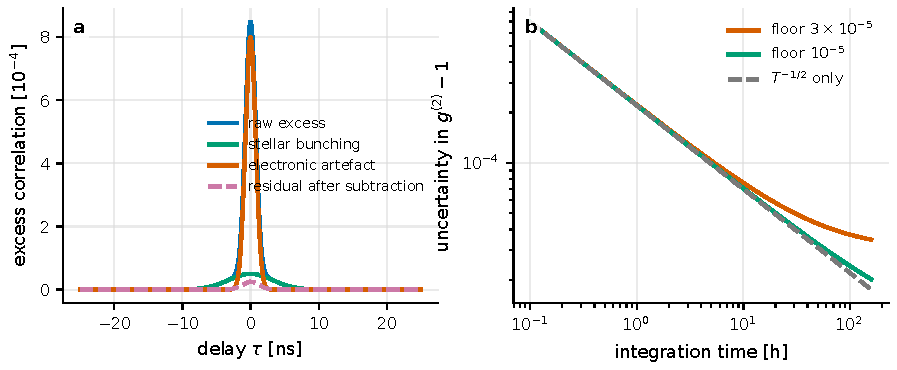
\includegraphics[width=0.96\linewidth]{figures/generated/chapter_21/ch21_calibration_artifacts.pdf}
\caption{校准误差如何伪装成相关信号。左图里电子串扰峰比 \(5\times10^{-5}\) 的天体聚束峰高出一个量级以上；若模板扣除后还留下窄残差，就会污染 \(\hat g^{(2)}(0)\)。右图显示积分时间只把\emph{统计}误差按 \(T^{-1/2}\) 压低；一旦存在 \(10^{-5}\)--\(3\times10^{-5}\) 的系统地板，再积分也不能自动改善结论。}
\label{fig:e27-calibration}
\end{figure}

对付系统项的正确姿势不是"积得更久"，而是设计一整套零检验（null test），让"真信号"和"伪信号"在不同操作下表现不同：时间平移（time-shift）把一路事件整体挪动远大于相关宽度的时间，真正的天体峰应当消失，慢漂移和背景结构则应保留；离源（off-source）或离带（off-band）把视场或频段换到不含目标的地方，零延迟峰不应保留；通道置换把本不该相关的探测器、偏振或谱通道交叉相关，若仍有峰，优先怀疑串扰；分块收敛把数据切成多段，相关幅度的均值应稳定，误差应按 \(T^{-1/2}\) 下降\emph{直到}撞上地板。Guerin 的报告指出，TDC 伪相关若不扣除会让信噪比提前饱和；AQuEye/IquEye 文献也明确列出 SPAD 死时间、光纤延迟、环境控制对系统误差的贡献 \citep{2017MNRAS.472.4126G,2016SPIE.9907E..0NZ,1996ApOpt..35.1956C,2013NIMPA.725..187J,2020RScI...91a3108W}。

收束：\textbf{强度干涉免掉的是大气相位，不是校准；信号既然被稀释到 }\(\mathbf{10^{-5}}\)\textbf{，就必须假设同量级的仪器伪相关一直在场，用零检验而不是用更长积分去对付它。}


\section{"没有相位"为什么不等于"不能成像"}
\label{sec:e27-phase}

第四个坑来自一句听上去很有道理的话："强度干涉丢了相位，所以只能测直径，不能成像。"前半句对，后半句错。

先把对的部分说清楚。第 \ref{chap:e10} 章的 van Cittert--Zernike 定理告诉我们，天体亮度分布 \(I(\boldsymbol\theta)\) 的角傅里叶变换就是复可见度 \(V(u,v)\)——它既有模又有相位。振幅干涉直接测这个复数 \(V\)；而强度干涉测的是两路强度相关，拿到的是模平方 \(|V(u,v)|^2\)，\textbf{一阶复可见度的相位确实丢掉了}。这是真实的信息损失，不能装作没有。

但"丢了相位"绝不等于"什么结构都测不出"。\(|V|^2\) 里仍然含着大量信息：均匀圆盘的直径、边缘昏暗（limb darkening）的程度、双星的间距与亮度比、旋转扁星的椭率、简单盘面的尺度，全都可以直接用 \(|V|^2\) 对 \(u,v\) 的依赖去拟合出来。第 \ref{chap:e11} 章讲从可见度到成像时，做的就是这件事。丢相位真正带来的困难，是一类特定的\textbf{退化}（degeneracy），其中最干净的一个是镜像退化。

镜像退化的道理，一行代数就能说透。设想把亮度分布整体做点对称反演，\(I(\boldsymbol\theta)\to I(-\boldsymbol\theta)\)。傅里叶变换有一条基本性质：函数做点对称反演，其频谱取复共轭。记原亮度 \(I(\boldsymbol\theta)\) 的复可见度为 \(V(\boldsymbol u)\)（即 \(V=\widetilde I\)），那么反演后的亮度 \(I(-\boldsymbol\theta)\) 其可见度为
\[
  \mathcal V_{I(-\boldsymbol\theta)}(\boldsymbol u)
  \equiv\widetilde{I(-\boldsymbol\theta)}(\boldsymbol u)
  =V^\ast(\boldsymbol u).
\]
于是取模平方，
\[
  \big|\mathcal V_{I(-\boldsymbol\theta)}(\boldsymbol u)\big|^2
  =\big|V^\ast(\boldsymbol u)\big|^2=\big|V(\boldsymbol u)\big|^2.
\]
两者\emph{完全相同}。这意味着：一个天体和它的镜像，产生的 \(|V|^2\) 一模一样，强度干涉\emph{原理上}就无法把它们分开——分开二者所需的方向信息，恰好藏在被丢掉的可见度相位符号里。第 \ref{chap:e11} 章已经画过这个相位缺失问题，图 \ref{fig:e27-phase-loss} 用一个不等亮双源和它的镜像再演示一次。

\begin{figure}[tbp]
\centering
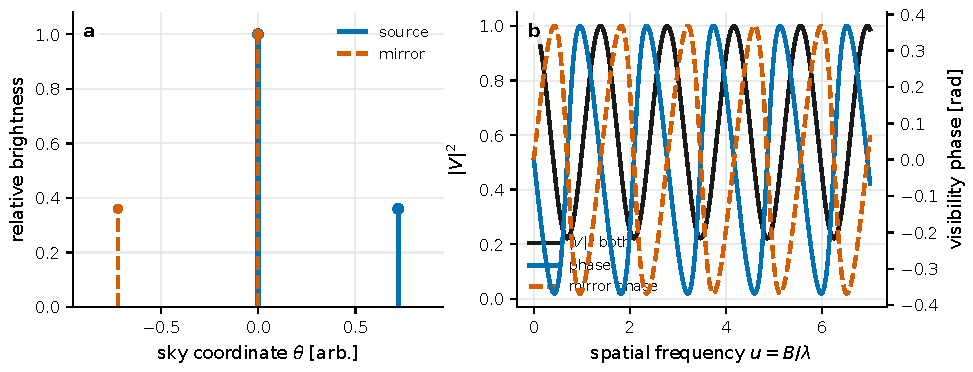
\includegraphics[width=0.96\linewidth]{figures/generated/chapter_21/ch21_phase_loss.pdf}
\caption{只测 \(|V|^2\) 带来的镜像退化。左图是一个不等亮双源和它的点对称镜像；右图显示二者的 \(|V|^2\) 完全重合，差别只在可见度相位的符号。强度干涉能约束结构，但要补回丢失的方向信息，得靠多基线覆盖、模型先验或高阶相关。}
\label{fig:e27-phase-loss}
\end{figure}

要把镜像、非对称结构、复杂形态区分开，正确的做法不是抱怨"没相位"，而是补信息：铺开多基线、加物理先验、用带正则化的相位反演（phase retrieval），或者引入三阶强度相关等高阶信息 \citep{2003RPPh...66..789M,2009A&A...507.1719F,2012NewAR..56..143D,2014MNRAS.437..798M,2022MNRAS.512.1722K}。其中三阶相关值得单说一句，因为它常被过度承诺：理想情况下，三阶强度相关能给出类似闭合相位（closure phase）的信息，从而部分补回方向；但它的信号比二阶相关\emph{更弱}。如果二阶相关的统计误差已经贴着上一节的系统地板，三阶相关会被同一批光子率和同一套校准问题卡得更死。所以三阶相关是大型阵列、极亮目标的探索方向，而第一代科学案例（第 \ref{chap:e25} 章）通常更务实——先从 \(|V|^2\) 的少参数模型做起，再逐步加先验做成像。

收束：\textbf{强度干涉丢的是可见度\emph{相位}，不是全部结构；}\(\mathbf{|V|^2}\)\textbf{ 足以约束直径、双星、扁率等许多量，真正丢掉的是区分镜像的方向信息，要靠多基线、先验或高阶相关补回。}


\section{量子超分辨为什么不能随意突破衍射}
\label{sec:e27-superres}

第五个坑，恰好长在一项真实成果的旁边，所以格外容易掉进去。SPADE（spatial-mode demultiplexing，空间模式解复用）纠正的是一个货真价实的统计误解：\textbf{Rayleigh 判据并不是所有参数估计问题的信息极限}。第 \ref{chap:e12} 章一步不跳地证明过：对两个弱、等亮、互不相干的点源，当角间距 \(s\) 远小于点扩散函数宽度 \(\sigma\) 时，直接成像对 \(s\) 的 Fisher 信息（Fisher information）以 \(s^2\) 的速度掉到零（这就是所谓的"Rayleigh 诅咒"），而理想的空间模式排序能把每光子的 Fisher 信息保持在有限值 \citep{2015Optic...2..646T,2016PhRvX...6c1033T,2016OExpr..24.3684N,2017PhRvL.118g0801T}。这是真结论，别打折。

但恰恰因为它是真的，才更要防止被夸张成"量子超分辨能任意突破衍射、能从几个光子里重建任意复杂图像"。要看清边界，回到第 \ref{chap:e12} 章的 Cramér--Rao 下界（Cramér--Rao bound）。任何无偏估计量 \(\hat s\) 的方差满足
\begin{equation}
  \operatorname{Var}(\hat s)\;\ge\;\frac{1}{N_\gamma\,F_s},
  \label{eq:e27-crb}
\end{equation}
\begin{formulaexplain}
\(\hat s\) 是对角间距的估计，\(N_\gamma\) 是进入正确模式分析的光子数，\(F_s\) 是\emph{每个光子}对 \(s\) 的 Fisher 信息。测量方式只能改 \(F_s\)，改不了 \(N_\gamma\)；下界要真达到，还得没有背景、像差和模式串扰。
\end{formulaexplain}

逐符号落实。\(s\) 是待估的角间距，单位可用 rad、mas，或直接以 PSF 宽度 \(\sigma\) 归一化；\(N_\gamma\) 是无量纲的有效光子数——注意是\emph{进入了正确模式分析}的光子数，不是打到望远镜上的总光子数；\(F_s\) 是每光子 Fisher 信息，量纲是角度的 \(-2\) 次方。式 \eqref{eq:e27-crb} 把三件事一次讲明白：第一，SPADE 提高的是 \(F_s\)（把 \(s^2\to0\) 的坍塌堵住），它\textbf{替代不了 }\(N_\gamma\)——光子数太少，方差照样爆炸；第二，下界是"\(\ge\)"，是可能达到的\emph{最好}情形，\textbf{量子下界不会自动可达}，背景、像差、模式串扰、质心（centroid）误差每一样都会让实际方差高于这条线；第三，把两点源的结论套到任意复杂图像上是没有根据的。图 \ref{fig:e27-superresolution} 左边画出模式排序确实把误差标度大幅拉低，但一道 \(0.003\sigma\)--\(0.01\sigma\) 的模式/质心误差地板会终止改善；右边用一个玩具模型显示，想恢复更高阶的矩或模式，所需光子数会\emph{急剧}上升。

\begin{figure}[tbp]
\centering
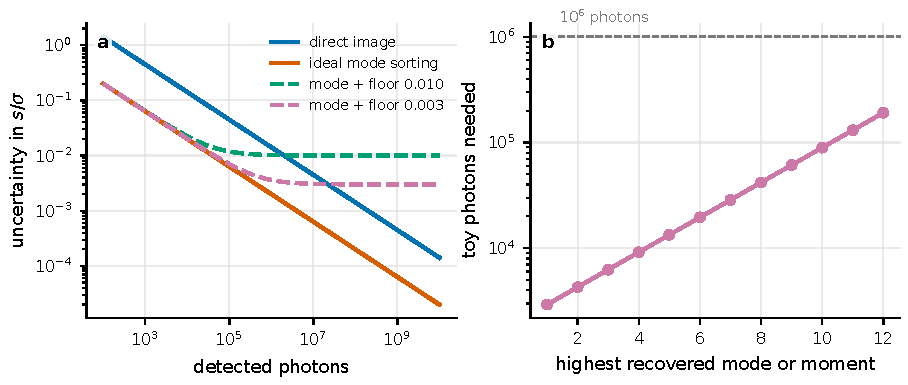
\includegraphics[width=0.96\linewidth]{figures/generated/chapter_21/ch21_superresolution_budget.pdf}
\caption{量子超分辨的光子预算与系统地板。左图取 \(s=0.2\sigma\)，比较直接成像与理想模式排序的统计误差标度：模式排序显著降低误差，但 \(0.003\sigma\)--\(0.01\sigma\) 的模式/质心误差地板会让改善停下来。右图用玩具模型显示，恢复更高阶矩或模式所需的光子数快速上升——复杂图像不可能从少数光子里任意恢复。}
\label{fig:e27-superresolution}
\end{figure}

天文语境里还有一层更细的条件常被忽略：源本身的相干性，以及传播之后的一阶空间相干。SPADE 的干净结论是对"两点\emph{互不相干}高斯源"证的；一旦源是部分相干（partially coherent）的，模式概率会改变，Rayleigh 诅咒是否重新出现，学界的讨论正是围绕这个条件展开 \citep{2017NJPh...19b3054T,2017PhRvA..95f3847A,2018Optic...5.1177P,2018Optic...5.1382L,2019Optic...6..400T}。因此，把"两点非相干高斯源"的结论直接搬到星系、吸积盘、喷流或强透镜弧上，会悄悄丢掉适用条件。

收束：\textbf{Rayleigh 判据不是估计极限，这是 SPADE 的真本事；但式 }\eqref{eq:e27-crb}\textbf{ 里的量子下界既需要足够的 }\(\mathbf{N_\gamma}\)\textbf{、又不会自动可达，脱离"两点、非相干、无背景、模式对齐"这些条件，超分辨就只剩一个口号。}


\section{天体 laser、maser 与非泊松统计最容易混在哪里}
\label{sec:e27-maser}

第六个坑集中在天体受激辐射源上，而且是好几条误会拧在一起。最典型的一句是："天体 laser/maser 一定给 \(g^{(2)}=1\)。"

先拆第一层：\textbf{高亮温（high brightness temperature）不等于相干态}。受激辐射能产生极高的亮温、极窄的谱线、很强的偏振——这些是 maser（microwave amplification by stimulated emission，微波受激辐射放大）的招牌。但招牌不等于内在统计。实验室激光之所以逼近相干态，靠的是稳定的谐振腔加饱和增益把强度涨落钳住；天体环境里根本没有这样的腔。第 \ref{chap:e06} 章分清过：相干态是一个很特殊的量子态，它的指纹是\emph{泊松}光子数分布，而不是"亮"或"窄"。一条谱线又亮又窄，完全可能仍带着很强的强度涨落——亮温、线宽、偏振是"多亮多窄多整齐"的度量，光子统计是"涨落多大"的度量，两把尺子量的是不同的东西。未饱和 maser、饱和 maser、速度相干路径、泵浦（pump）涨落、多个斑点叠加、连续谱背景，每一样都会改写光子统计 \citep{1982RvMP...54.1225E,1992ARA&A..30...75E,1985ARA&A..23..169D}。Eta Carinae 的 Weigelt blobs 里，Fe II 和 O I 线的自然激光候选，就要同时看 Ly\(\alpha\) 泵浦、能级反转、线宽、空间位置和连续谱扣除才能定性；Brown--Twiss--Townes 外差相关甚至被提出来专门去测那条极窄 Fe II 线的线宽 \citep{2004A&A...428..497J,2005MNRAS.364..731J,2005NewA...10..361J,2008AIPC..984..216D}。

第二层是混合稀释，值得把公式一步不跳地推出来。设观测到的光由若干独立成分叠加，总强度 \(I=\sum_a I_a\)，不同成分之间没有强度相关。零延迟的二阶相干是
\[
  g^{(2)}_{\rm mix}(0)=\frac{\langle I^2\rangle}{\langle I\rangle^2}.
\]
先算分子。展开 \(I^2=\big(\sum_a I_a\big)^2=\sum_a I_a^2+\sum_{a\ne b}I_aI_b\)，取平均：
\[
  \langle I^2\rangle
  =\sum_a\langle I_a^2\rangle
  +\sum_{a\ne b}\langle I_a\rangle\langle I_b\rangle,
\]
其中交叉项用了"不同成分无相关"这条假设，把 \(\langle I_aI_b\rangle\) 拆成 \(\langle I_a\rangle\langle I_b\rangle\)。再用每个成分自己的定义 \(\langle I_a^2\rangle=g_a^{(2)}(0)\langle I_a\rangle^2\)，并把交叉求和补全成完整双重求和再减去对角：
\[
  \sum_{a\ne b}\langle I_a\rangle\langle I_b\rangle
  =\Big(\sum_a\langle I_a\rangle\Big)^2-\sum_a\langle I_a\rangle^2
  =\langle I\rangle^2-\sum_a\langle I_a\rangle^2.
\]
合起来：
\[
  \langle I^2\rangle
  =\sum_a g_a^{(2)}(0)\langle I_a\rangle^2
  +\langle I\rangle^2-\sum_a\langle I_a\rangle^2.
\]
两边除以 \(\langle I\rangle^2\)，并记通量分数 \(f_a=\langle I_a\rangle/\langle I\rangle\)：
\[
  g^{(2)}_{\rm mix}(0)
  =\sum_a g_a^{(2)}(0)f_a^2+1-\sum_a f_a^2.
\]
把 1 挪到左边，右边按 \(f_a^2\) 合并，得到干净的结果：

\begin{equation}
  g^{(2)}_{\rm mix}(0)-1
  =\sum_a f_a^2\left[g_a^{(2)}(0)-1\right],
  \qquad
  f_a=\frac{\langle I_a\rangle}{\sum_b\langle I_b\rangle}.
  \label{eq:e27-mixture}
\end{equation}
\begin{formulaexplain}
\(f_a\) 是第 \(a\) 个成分的通量分数（无量纲，各成分之和为 1）。关键在那个\emph{平方}：相关超额按 \(f_a^2\) 加权，所以一点点热连续谱或多成分混合，就能把 \(g^{(2)}\) 的解读搅乱。
\end{formulaexplain}

那个平方是全部要害。代个数字：一个只占总通量 \(20\%\) 的热成分，即使它自己满格 \(g_a^{(2)}(0)-1=1\)，混进来后也只贡献 \(f_a^2\times1=0.2^2=0.04\) 的对比度；若这个热成分再摊到 \(M=100\) 个模式、\(\tau_c/\Delta t=10^{-5}\)，观测对比度就成了 \(0.04\times10^{-5}/100\sim4\times10^{-9}\)——彻底沉底。反过来，一条未饱和的受激线若带着泵浦强度噪声，可能给出\emph{超}泊松（super-Poisson）统计；但这种结果得先把谱线、连续谱、仪器响应分离干净，绝不能一见 \(g^{(2)}>1\) 就归给新物理。图 \ref{fig:e27-maser} 把这两条分支画在一起。

\begin{figure}[tbp]
\centering
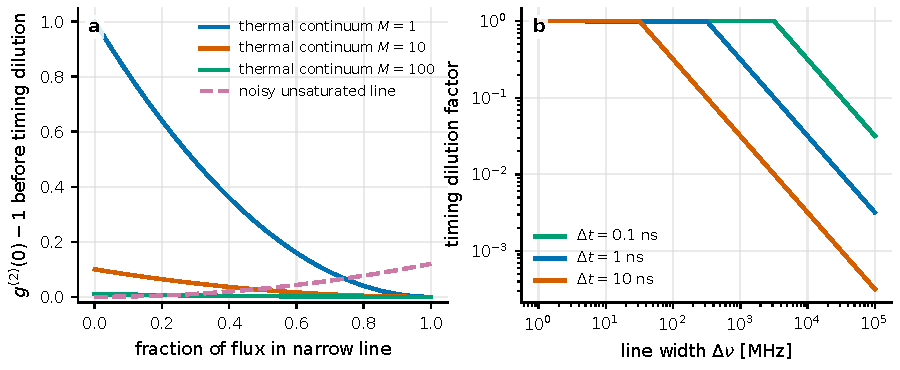
\includegraphics[width=0.96\linewidth]{figures/generated/chapter_21/ch21_maser_mixed_statistics.pdf}
\caption{天体 maser/laser 候选中的混合统计。左图显示窄线通量分数增大时，热连续谱的聚束按 \(f_a^2\) 被稀释；若窄线本身带未饱和强度噪声，则冒出另一条超泊松分支。右图显示谱线宽度和电子学时间箱对相关对比度的稀释——MHz--GHz 的线宽需要 ns 甚至更快的时间响应，才能保住可观的峰值。}
\label{fig:e27-maser}
\end{figure}

第三层：非泊松统计有太多\emph{普通}来源，别急着往量子光源上想。最典型的是把随机变源当成 Cox 过程（Cox process，又称双随机泊松过程）：给定瞬时率 \(\Lambda\) 时计数服从泊松，但 \(\Lambda\) 自己随时间或环境涨落。用全方差公式（law of total variance，把方差拆成"条件方差的期望"加"条件期望的方差"）算一算，记 \(\Lambda\) 为一个箱里的期望计数，泊松条件下 \(\operatorname{Var}(N\mid\Lambda)=\Lambda\)、\(\mathbb E(N\mid\Lambda)=\Lambda\)，于是
\[
  \operatorname{Var}(N)
  =\mathbb E[\operatorname{Var}(N\mid\Lambda)]+\operatorname{Var}(\mathbb E[N\mid\Lambda])
  =\mathbb E(\Lambda)+\operatorname{Var}(\Lambda),
\]
而 \(\mathbb E(N)=\mathbb E(\Lambda)\)。两者相除即得 Fano 因子（Fano factor）：

\begin{equation}
  F_{\rm Fano}
  \equiv\frac{\operatorname{Var}(N)}{\mathbb E(N)}
  =1+\frac{\operatorname{Var}(\Lambda)}{\mathbb E(\Lambda)}.
  \label{eq:e27-fano}
\end{equation}
\begin{formulaexplain}
\(F_{\rm Fano}\) 是计数方差与均值之比（纯泊松等于 1）。只要瞬时率 \(\Lambda\) 自己在涨落，计数就自然变成超泊松（\(F>1\)），根本不必先请出非经典光源。
\end{formulaexplain}

也就是说，只要源在变，\(F_{\rm Fano}\) 在合适的箱宽下就\emph{必然}大于 1，这是最平凡的超泊松。仪器还会从反方向捣乱：死时间会压掉挨得太近的事件，让短延迟出现负相关、把 \(F_{\rm Fano}\) 压到 1 以下（欠离散，under-dispersion）；afterpulsing（余脉冲）则会在探测器特征时间之后制造正相关。第 \ref{chap:e07} 章给过的 afterpulsing 概率 \(10^{-4}\)--\(10^{-2}\)，已经足以污染许多短延迟搜索。所以在喊"非泊松"之前，先把这几张诊断图画全：Fano 因子随箱宽的变化、短延迟自相关与互相关、暗场数据、离源数据、时间平移背景。图 \ref{fig:e27-nonpoisson} 把这些普通来源的不同标度并排画了出来。

\begin{figure}[tbp]
\centering
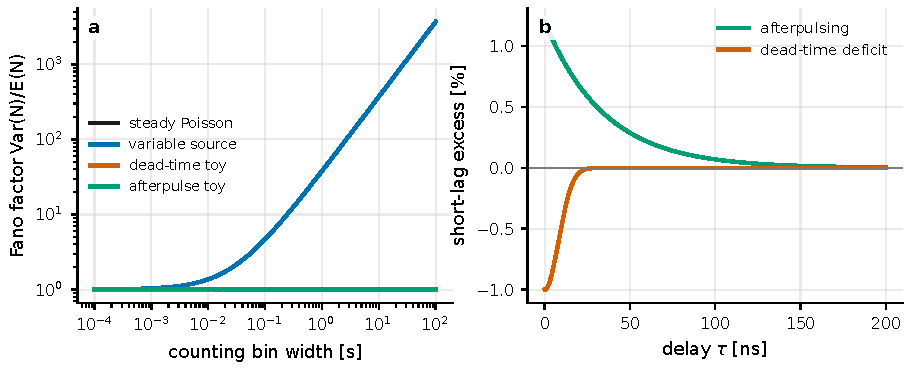
\includegraphics[width=0.96\linewidth]{figures/generated/chapter_21/ch21_nonpoisson_diagnostics.pdf}
\caption{非泊松统计的普通来源。左图用 Fano 因子展示稳态泊松、慢变源、死时间和 afterpulsing 各自不同的标度：慢变源在长箱里变成超泊松，死时间造成欠离散。右图显示 afterpulsing 与死时间在短延迟相关函数里的相反形状——这些仪器特征应先从暗场和交叉通道里量化出来。}
\label{fig:e27-nonpoisson}
\end{figure}

收束：\textbf{亮、窄、偏振强都不等于相干态；混合光按 }\(\mathbf{f_a^2}\)\textbf{ 稀释相关，变源与死时间、余脉冲会自然造出非泊松统计——把它们排除干净之前，任何"非泊松"都不该记在新物理头上。}


\section{假警报如何伪造出"新物理"的边界}
\label{sec:e27-false-alarm}

最后一个坑，是所有搜索类工作的通病：把一次小概率事件当成发现。

问题的根子是"多重检验"（multiple testing）。设一次检验偶然给出如此极端结果的尾概率是 \(p_0\)，而你独立地做了 \(N_{\rm trial}\) 次检验，那么"至少出现一次"这种偶然峰的概率是多少？逐步算：单次\emph{不}出现的概率是 \(1-p_0\)，\(N_{\rm trial}\) 次全都不出现是 \((1-p_0)^{N_{\rm trial}}\)（用了各次独立），于是至少出现一次是

\begin{equation}
  p_{\rm any}=1-(1-p_0)^{N_{\rm trial}}
  \simeq N_{\rm trial}\,p_0
  \qquad(N_{\rm trial}\,p_0\ll1).
  \label{eq:e27-trials}
\end{equation}
\begin{formulaexplain}
\(p_0\) 是单次检验的尾概率，\(N_{\rm trial}\) 是试验次数。搜索空间越大，偶然撞见一次高峰的概率越高，所以要报告\emph{全局}显著性，而不是单次的 \(p_0\)。
\end{formulaexplain}

那个约等号来自一步标准展开：当 \(p_0\) 很小、\emph{且} \(N_{\rm trial}p_0\ll1\) 时，\((1-p_0)^{N_{\rm trial}}\approx e^{-N_{\rm trial}p_0}\approx1-N_{\rm trial}p_0\)（先用 \(\ln(1-p_0)\approx-p_0\)，再对指数做一阶泰勒展开），代回即得 \(p_{\rm any}\approx N_{\rm trial}p_0\)。务必记住这条近似\textbf{只在 }\(\mathbf{N_{\rm trial}p_0\ll1}\)\textbf{ 时成立}；一旦搜索空间大到 \(N_{\rm trial}p_0\gtrsim1\)，就不能再用它，得回到未近似的 \(p_{\rm any}=1-(1-p_0)^{N_{\rm trial}}\approx1-e^{-\mu}\)，其中我们记
\[
  \mu\equiv N_{\rm trial}\,p_0
\]
为偶然峰的\textbf{期望个数}（无量纲，可以远大于 1），而概率 \(p_{\rm any}=1-e^{-\mu}\) 始终落在 \(0\) 与 \(1\) 之间。这个 \(N_{\rm trial}\) 可以从四面八方冒出来：时间箱数、频率通道数、基线数、目标数、模型网格点数，甚至事后才圈定的窗口。代个数字体会一下：若每晚扫描 \(10^6\) 个候选的延迟/频率/目标组合，一个单次 \(p_0=10^{-5}\)（听起来已经"很显著"）的事件，其偶然峰的期望个数是
\[
  \mu=N_{\rm trial}\,p_0\simeq10^{6}\times10^{-5}=10,
\]
于是全局出现的概率是
\[
  p_{\rm any}=1-e^{-\mu}\approx1-e^{-10}\approx0.99995\approx1,
\]
几乎必然——意思是每晚平均约有 \(\mu\approx10\) 个这样的"惊人峰"冒出来，纯属搜索空间的自然尾部。这里要特别把两件事分清：\(10\) 是期望\emph{个数} \(\mu\)，不是概率；把它写成 \(p_{\rm any}=10\)（并顺手把只在 \(\mu\ll1\) 时成立的近似式 \(p_{\rm any}\approx N_{\rm trial}p_0\) 硬套到 \(\mu=10\) 上）正是本节要教你避开的典型错误——概率永远不会超过 1，超过 1 的那个量一定是计数的期望值。图 \ref{fig:e27-false-alarm} 左边画出 \(\mu=8\) 的单个泊松箱偶尔会甩出 \(N\ge17\) 的高计数尾，右边画出同一个单次 \(p_0\) 在大量试验后如何滚成很高的全局假警报概率。

\begin{figure}[tbp]
\centering
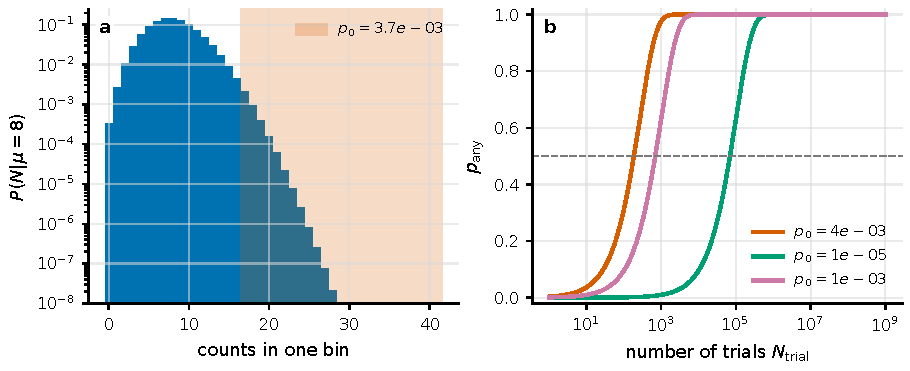
\includegraphics[width=0.96\linewidth]{figures/generated/chapter_21/ch21_poisson_false_alarm.pdf}
\caption{泊松尾部与多重检验。左图里 \(\mu=8\) 的单个箱偶尔会出现 \(N\ge17\) 的高计数尾；右图显示同样的单次 \(p_0\) 在大量试验中如何变成很高的全局假警报概率。事件表搜索、周期搜索、跨频相关、暂现源筛选，都必须报告 \(N_{\rm trial}\) 或等效的全局显著性。}
\label{fig:e27-false-alarm}
\end{figure}

顺带纠正一个更大的语义误会：\textbf{"量子天文学"不等于"量子引力"}。本书前面绝大部分内容研究的是光场统计、模式测量、相干函数、仪器和信息极限——都是可测的地面物理。黑洞、CMB、轴子、宇宙双折射、暗物质透镜之所以能进这条主线，是因为它们能被写成\emph{可观测}的时间、频率、偏振或空间相关量，而不是因为每个话题都得动用普朗克尺度物理。一个真正可检查的异常，第一步永远是把数据来源拆开：
\begin{equation}
  d_{\rm obs}=d_{\rm sky}(\boldsymbol\theta)
  +d_{\rm inst}(\boldsymbol\phi)
  +d_{\rm sel}(\boldsymbol\psi)
  +n.
  \label{eq:e27-data-model}
\end{equation}
\begin{formulaexplain}
\(d_{\rm obs}\) 是观测数据（延迟直方图、\(|V|^2\)、偏振相关或事件时间）；右边把天空模型、仪器模型、选择函数和噪声分开。任何"新物理"解释都得先证明前面这些普通项\emph{解释不了}数据。
\end{formulaexplain}

其中 \(d_{\rm sky}(\boldsymbol\theta)\) 是天体模型（参数 \(\boldsymbol\theta\)），\(d_{\rm inst}(\boldsymbol\phi)\) 是仪器模型，\(d_{\rm sel}(\boldsymbol\psi)\) 是选择函数，\(n\) 是噪声。只要这四项还没分开，异常峰、偏振旋转或超泊松计数就都不该直接归因于新物理——它们更可能藏在 \(d_{\rm inst}\) 或 \(d_{\rm sel}\) 里。这也正好接上第 \ref{chap:e28} 章：一份研究计划的最后一页，应当回到"新增的观测量到底是什么"——是平均强度、二阶相关、跨频协方差、偏振相关，还是模式计数；每个量都要配上单位、典型范围、适用条件（热光、高斯 PSF、弱光、少参数源模型、稳定仪器响应），并至少从时间平移、离源、离带、暗场、错偏振、注入恢复里挑两个零检验，把全局显著性和系统误差地板\emph{一起}写进结论。

收束：\textbf{搜索空间越大，偶然的"显著峰"越是必然；不报告 }\(\mathbf{N_{\rm trial}}\)\textbf{ 的显著性没有意义，而"量子天文学"的门槛是可观测的相关量，不是普朗克尺度的新物理。}


\section{本章要点}
\label{sec:e27-summary}

\begin{itemize}
  \item \textbf{数光子只是拿到原料。}真正的量子信息在事件之间的联合分布里；若时间、探测器、频率、偏振标签不进模型，再精密的单光子计数也还是经典测光。"少光子"与"量子"是两把尺子。
  \item \(\mathbf{g^{(2)}\simeq1}\)\textbf{ 什么也证明不了。}热光的聚束峰被有效模式数 \(M_{\rm eff}\)（含 \(\Delta t_{\rm eff}/\tau_c\)）稀释到 \(10^{-5}\)--\(10^{-6}\) 是常态，见式 \eqref{eq:e27-dilution}。唯一过硬的非经典判据是反聚束 \(g^{(2)}(0)<1\)，经典光做不到。
  \item \textbf{强度干涉不怕相位，但怕校准。}信号既已稀释到 \(10^{-5}\)，就得假设同量级的仪器伪相关一直在场（式 \eqref{eq:e27-calibration-model}）。系统地板不随 \(T^{-1/2}\) 下降，靠零检验而非更长积分来对付。
  \item \(\mathbf{|V|^2}\)\textbf{ 丢的是相位，不是结构。}直径、双星、扁率都能拟合，真正丢的是区分镜像的方向信息（\(|V^\ast|^2=|V|^2\)），要靠多基线、先验或高阶相关补回。
  \item \textbf{量子超分辨有边界。}Rayleigh 判据确实不是估计极限，但式 \eqref{eq:e27-crb} 的量子下界既要足够光子 \(N_\gamma\)、又不会自动可达；离开"两点、非相干、无背景、模式对齐"就只剩口号。
  \item \textbf{亮窄偏振强不等于相干态。}混合光按 \(f_a^2\) 稀释相关（式 \eqref{eq:e27-mixture}），变源（Cox 过程，式 \eqref{eq:e27-fano}）、死时间、余脉冲都会自然造出非泊松统计——排除干净前不算新物理。
  \item \textbf{搜索必报全局显著性。}偶然峰随 \(N_{\rm trial}\) 线性增多（式 \eqref{eq:e27-trials}）；异常要先按天空/仪器/选择/噪声四项拆开（式 \eqref{eq:e27-data-model}），才谈得上新物理。
\end{itemize}

\medskip
\noindent\textbf{想一想。}
\begin{itemize}
  \item 你在 \(500\,{\rm nm}\)、\(5\,{\rm nm}\) 带宽下用 \(2\,{\rm ns}\) 的相关箱测一颗恒星的热光。单模情形下，你预期测到的 \(g^{(2)}_{\rm meas}(0)-1\) 大概是什么量级？（提示：先算 \(\tau_c\)，再用式 \eqref{eq:e27-dilution}。）
  \item 一次谱线搜索里，你在 \(3\times10^{5}\) 个频率通道中找到一个单次 \(p_0=3\times10^{-6}\) 的峰。它的全局假警报概率是多少？你会宣布发现吗？
  \item 有人报告某天体 maser 的 \(g^{(2)}(0)=1.5\)，声称是非经典光。在相信之前，你会先要求他排除哪三种普通来源？
\end{itemize}
